\documentclass[11pt,a4paper]{article}
\usepackage[T1]{fontenc}
\usepackage{mathpazo}
\usepackage[scaled=.90]{helvet}
\usepackage[a4paper,left=26mm,right=26mm,top=22mm,bottom=22mm,headheight=13pt]{geometry}
\usepackage{amsmath,amssymb,graphicx,xcolor,booktabs,array,fancyhdr,microtype}
\usepackage{hyperref}
\definecolor{ink}{HTML}{202B35}
\definecolor{accent}{HTML}{185E64}
\definecolor{muted}{HTML}{53636B}
\hypersetup{colorlinks=true,allcolors=accent,pdftitle={A 56.07936-day recurrence at TIC 153838604},pdfsubject={Archival eclipse photometry and companion constraints, 20 November 2026}}
\graphicspath{{figures/}}
\pagestyle{fancy}\fancyhf{}
\fancyhead[L]{\scriptsize\sffamily\color{muted} TIC 153838604}
\fancyhead[R]{\scriptsize\sffamily\color{muted} Eclipse timing and companion constraints}
\fancyfoot[C]{\small\sffamily\color{muted}\thepage}
\renewcommand{\headrulewidth}{.25pt}
\setlength{\parindent}{1em}
\setlength{\parskip}{1.5pt}
\setlength{\emergencystretch}{1.5em}
\setlength{\abovedisplayskip}{6pt}\setlength{\belowdisplayskip}{6pt}
\newcommand{\Sec}[2]{\par\vspace{9pt}\noindent{\large\bfseries\sffamily\color{accent}#1\quad #2}\par\nobreak\vspace{3pt}\noindent\ignorespaces}
\newcommand{\Sub}[1]{\par\vspace{5pt}\noindent{\bfseries #1}\enspace\ignorespaces}
\newcommand{\captext}[2]{\par\nobreak\vspace{3pt}\noindent\begin{minipage}{\linewidth}\small\sffamily\raggedright\textbf{#1.}\enspace #2\end{minipage}\par\vspace{4pt}}
\newcommand{\Rp}{R_{\mathrm p}}
\newcommand{\Rj}{R_{\rm J}}
\newcommand{\Mj}{M_{\rm J}}
\newcommand{\kms}{\mathrm{km\,s^{-1}}}
\newcommand{\btjd}{\mathrm{BTJD}}
\newcommand{\urlname}[2]{\href{#1}{#2}}
\newcommand{\entry}[2]{\par\noindent\hangindent=2.2em\hangafter=1\makebox[2.2em][l]{[#1]}#2\par}
\begin{document}
\thispagestyle{plain}
\noindent{\fontsize{21.5}{24.5}\selectfont\bfseries A 56.07936-day recurrence at TIC~153838604}\par
\vspace{4pt}
\noindent{\large\sffamily\color{muted}Eclipse timing and archival constraints on the companion}\par
\vspace{3pt}\noindent{\small\sffamily\color{muted}20 November 2026}\par
\vspace{10pt}
\noindent\rule{\linewidth}{.6pt}\par\vspace{3pt}
\noindent\textbf{Abstract.}
Hawthorn et al. identified two transit-like events toward TIC~153838604 separated by 729 days. We recover two further eclipses in TESS sectors 97 and 98, on 22 October and 17 December 2025. The four midpoints follow a 56.07936-day photometric period over seven years, with a maximum residual of 3.2 minutes. Independent difference images on two detectors locate the lost flux within 0.08 pixel of the target. At phase 0.5 of this period, three TESS observing windows give a nominal one-sided 95\% upper limit of 0.71 parts per thousand for a 2.5-hour triangular secondary eclipse. A grazing Jupiter-mass companion and a low-mass star can reproduce the primary light curve on eccentric orbits that miss secondary eclipse, while predicting radial-velocity semiamplitudes of 0.061 and 6.84 $\kms$, respectively. Four ASAS-SN $g$-band measurements support dimming at the predicted times but do not distinguish these models. A doubled orbital period with similar alternating eclipses also remains possible. The result is an ephemeris for a previously ambiguous signal and a quantitative description of the remaining companion ambiguity.\par
\vspace{3pt}\noindent\rule{\linewidth}{.3pt}
\Sec{1}{The observed eclipses}
TIC~153838604 (CTOI~153838604.01, Gaia DR3 4788303839668784896) is a $G=12.92$ star at ICRS coordinates $(68.07399^\circ,-47.60899^\circ)$. Hawthorn et al. [1] measured eclipses in 2018 and 2020 at BTJD 1447.10227 and 2176.13853. Throughout, $\btjd=\mathrm{BJD}_{\rm TDB}-2457000$, and 1 part per thousand (ppt) represents 0.1\% of the baseline flux. The original observations allowed several integer cycle counts. Two later TESS sectors sample additional eclipses on consecutive cycles (Fig.~1).
\begin{center}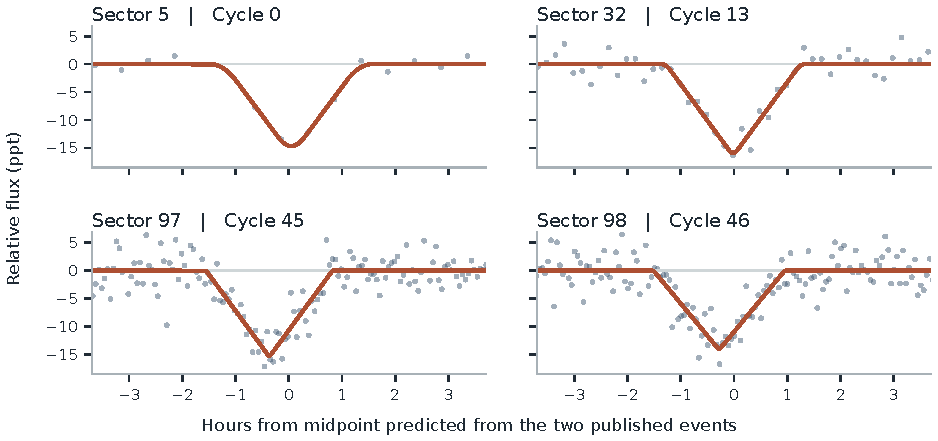
\includegraphics[width=.93\linewidth]{tess-eclipses.pdf}\end{center}
\captext{Figure 1}{Quality-selected TESS photometry around the four eclipses. The time origin in each panel is predicted from the published pair assuming 13 cycles between them. Red curves give independent, exposure-averaged triangular fits with local linear baselines. The last two events arrive 22 and 17 minutes earlier than this two-event prediction.}

\clearpage
\Sec{2}{Photometry, cycle count and localization}
The MIT Quick-Look Pipeline (QLP) provides TESS full-frame light curves [2,3] in sectors 4, 5, 31, 32, 97 and 98. We use cadences with zero quality flags and finite detrended flux. Sector 30 appears in a geometric footprint lookup, but its cutout spans detector columns 2121--2129, beyond the photosensitive range 45--2092. For each eclipse we fit a symmetric triangle and linear baseline within $\pm0.30$ day, integrating over the cadence duration. The triangle describes the timing and apparent depth of the measured V-shaped signal. We treat limb-darkened eclipse models separately in Section~4.
\begin{center}
\small\renewcommand{\arraystretch}{1.15}
\begin{tabular}{@{}rrrrrrr@{}}\toprule
Sector & Cycle $E$ & Cadence (s) & Midpoint (BTJD) & Depth (ppt) & Duration (h) & $O-C$ (min)\\\midrule
5  & 0  & 1800 & 1447.10424 & 16.27 & 2.53 & $-1.15$\\
32 & 13 & 600  & 2176.13788 & 16.44 & 2.53 & $+1.69$\\
97 & 45 & 200  & 3970.67403 & 15.48 & 2.38 & $-3.13$\\
98 & 46 & 200  & 4026.75736 & 14.21 & 2.47 & $+2.58$\\\bottomrule
\end{tabular}\end{center}
\captext{Table 1}{Independent eclipse fits to the default QLP aperture. $O-C$ is measured minus calculated midpoint under equation (1). Depth is the instantaneous fitted peak loss before averaging over each exposure.}
For the published separation of 729.03626 days, integer divisors 1 through 19 span the reported 38.37--729.04-day range. Divisor 13 predicts both later midpoints within 23 minutes. The next closest, divisor 15, misses them by 3.754 and 3.727 days. An equal-weight linear fit gives
\begin{equation}
T(E)\,[\mathrm{BJD}_{\rm TDB}]=2458447.10503+56.0793594\,E .
\end{equation}
Eclipse injections into 16, 35, 51 and 46 disjoint out-of-eclipse windows yield single-event timing errors of 1.75--2.16 minutes RMS. Propagating the larger of the regression and injection-derived period variances gives a one-standard-error scale of 0.000056 day. A Student-$t$ factor for two residual degrees of freedom gives an approximate 95\% allowance of 0.00024 day assuming stable shape, independent timing errors and a linear ephemeris.
\par For each divisor 2 through 18 of the fitted period there is at least one well-covered predicted additional eclipse. Across the selected windows, even with $\pm30$ minutes of timing allowance, the largest median core loss is 1.40 ppt. For divisors $\geq19$, at least one eclipse must occur inside BTJD 3997.0--4000.1, where the maximum over all possible centres is 2.55 ppt. The shallower 2025 event measures 8.90 ppt with the same core statistic. This excludes those shorter recurrences for comparably deep, isolated eclipses of similar duration.
\begin{center}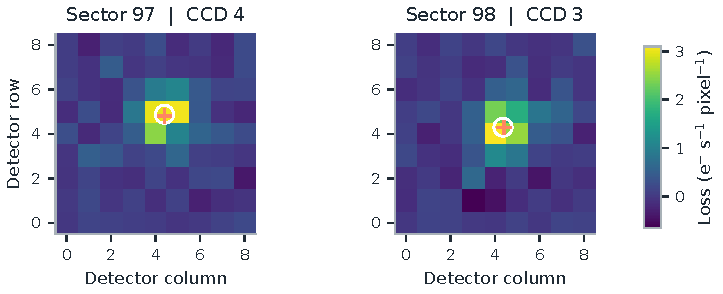
\includegraphics[width=.76\linewidth]{difference-images.pdf}\end{center}
\captext{Figure 2}{Flux lost per detector pixel in the two 2025 eclipses, with a fitted background plane removed. The catalogue positions (circles) and fitted loss centroids (crosses) differ by 0.079 and 0.044 pixel. Per-axis scatter measured by injections into comparison images is 0.07--0.11 pixel. Unresolved sources remain possible.}

\clearpage
\Sec{3}{Tests for secondary and alternating eclipses}
Under a 56.07936-day circular orbit, a secondary eclipse would fall near phase 0.5. Sectors 31, 97 and 98 contain well-sampled windows at this phase. We fit exposure-averaged triangular losses against a linear continuum. For 2.5-hour duration, the three measured peak depths are $-0.246$, $-0.181$ and $-0.015$ ppt, where positive denotes dimming. The inverse-variance combination is $-0.141$ ppt; undetrended aperture flux gives $-0.138$ ppt. Applying the same statistic to 34, 51 and 44 disjoint comparison windows yields 76,296 cross-sector assignments with 0.472 ppt scatter. Subtraction of the fifth noise percentile gives a nominal one-sided 95\% upper depth of 0.709 ppt. The data constrain a secondary of approximately the primary duration to less than about 5\% of the primary's observed depth at this phase.
\begin{center}\small\renewcommand{\arraystretch}{1.13}
\begin{tabular}{@{}crrr@{}}\toprule
Assumed duration & Phase-0.5 bound & \multicolumn{2}{c}{Unmasked phases with bounds below 5 ppt}\\
(h) & (ppt) & 56.079-day orbit & 112.159-day orbit\\\midrule
1.25 & 0.843 & 91.6\% & 71.5\%\\
2.50 & 0.709 & 95.4\% & 73.6\%\\
5.00 & 1.125 & 92.4\% & 67.4\%\\\bottomrule
\end{tabular}\end{center}
\captext{Table 2}{The fixed-phase calculation combines three sectors. At other phases, a single covered epoch is selected using its sector's comparison-window scatter, independently of the depth at that epoch. Percentages include unobserved trial centres in the denominator.}
The unknown-phase search tests a grid with ten-minute spacing and masks the identified eclipses. For the 2.5-hour template, 96.1\% of 7,903 unmasked phase trials at 56 days have data, and 63.8\% have at least two covered epochs. Conditional upper bounds use sector-matched comparison windows. The limits depend on shape, dilution and time sampling and are pointwise. In particular, they supply no simultaneous confidence band or survey-wide false-alarm probability for a target selected in a search across multiple stars and aliases.
\par If the orbital period is 112.15872 days, the deep eclipses occupy phases 0 and 0.5; the null windows above lie at quadrature. A simultaneous fit for epoch, slope and odd-event timing displacement gives $-1.4$ minutes, with injection-based 95\% interval $[-6.0,+4.1]$ minutes. The even-minus-odd duration difference is $+0.05$ h $[-0.33,+0.37]$ h; the default-aperture peak-depth difference is $-0.71$ ppt $[-2.58,+0.85]$ ppt. The small aperture gives $-3.08$ ppt, compared with $-0.04$ ppt in the large aperture. In sector 98 alone the fitted depth changes from 4.73 to 17.34 ppt between those apertures. Each event occurs in a distinct sector, so parity and aperture throughput are confounded. Window injections calibrate random and locally correlated errors under a specified shape. They do not absorb arbitrary sector-dependent dilution.
\Sec{4}{Geometrically viable companions}
For an illustrative $1.00\,M_\odot$, $0.9065\,R_\odot$ primary we fit quadratic limb-darkened eclipse profiles [4] to 632 local cadences, allowing a common impact parameter and projected speed and a linear baseline per sector. Eclipse times are fixed to the independent measurements. The example models adopt limb-darkening coefficients $(0.35,0.20)$, integrate over each exposure and use the nominal photometric period. Their mass and radius are assumed to demonstrate the light-curve degeneracy. No dynamical mass is measured.

\clearpage
\begin{center}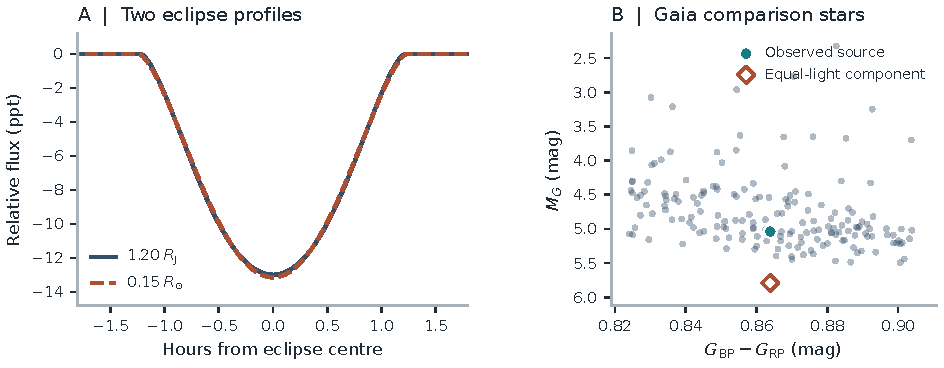
\includegraphics[width=.99\linewidth]{eclipse-models-cmd.pdf}\end{center}
\captext{Figure 3}{(A) Instantaneous primary-eclipse profiles for the example eccentric planet and stellar companion. The maximum difference at the actual integrated TESS cadences is 0.16 ppt. (B) Absolute Gaia $G$ magnitude versus colour for the target and 172 field stars. The diamond gives the component magnitude required if two identical stars contribute equally to the observed light.}
\begin{center}\small\renewcommand{\arraystretch}{1.15}
\begin{tabular}{@{}lrrrrrr@{}}\toprule
Companion model & $R_2/R_\star$ & $b_{\rm pri}$ & $e$ & $i$ & $b_{\rm sec}$ & $K_1$ ($\kms$)\\\midrule
$1\,\Mj$, $1.20\,\Rj$ & 0.1360 & 0.922 & 0.491 & $88.47^\circ$ & 2.702 & 0.061\\
$0.12\,M_\odot$, $0.15\,R_\odot$ & 0.1655 & 0.973 & 0.426 & $88.63^\circ$ & 2.414 & 6.84\\\bottomrule
\end{tabular}\end{center}
\captext{Table 3}{Illustrative 56-day solutions with periastron at primary conjunction ($\omega=90^\circ$). Companion-to-primary light ratios are assumed to be 0 and 0.001. Predicted primary-star velocity semiamplitudes are conditional on these adopted masses and orbits.}
The local speed inferred from an eclipse can exceed the circular speed for the adopted stellar density. For $\omega=90^\circ$ the ratio is $g=[(1+e)/(1-e)]^{1/2}$. Choosing $e=(g^2-1)/(g^2+1)$ realizes the two fitted speeds with eccentric Keplerian orbits. At superior conjunction $b_{\rm sec}=b_{\rm pri}(1+e)/(1-e)$ exceeds $1+R_2/R_\star$ in both examples. Exact orbital and constant-speed profiles agree within 4 ppm during eclipse. The illustrative models differ by $\Delta\chi^2=1.19$ under white-noise weighting. Correlated noise, uncertain dilution, stellar density and limb darkening preclude conversion of that difference into odds for the two masses.
\Sub{Gaia colour and luminosity.}
Gaia DR3 [5] gives $G=12.9243$, $G_{\rm BP}-G_{\rm RP}=0.8639$ and $\varpi=2.6468\pm0.0174$ mas. Direct inversion gives 377.8 pc and $M_G=5.038\pm0.014$ (parallax contribution alone), before extinction or zero-point corrections. Two identical stars at this distance would each require $M_G=5.790$. All 172 comparison stars within $3^\circ$, 300--500 pc and 0.04 mag of the target colour are brighter than that value; their median is 4.900 and their faintest is 5.492. This disfavors two ordinary equal-light stars at the catalogue distance. Extinction, metallicity, evolutionary state and unresolved hierarchical or background systems limit the inference.
\Sub{Astrometry and spectra.}
The renormalized unit weight error (RUWE) is 1.381, above a locally calibrated threshold of 1.238 [6]. Of 839 nearby stars of comparable magnitude and colour, 154 have RUWE at least this large. Gaia's aggregate velocity of $+75.61\pm2.03\,\kms$ combines 22 transits spanning 888 days. The faint-source processing combines cross-correlations; the catalogue uncertainty is not an epoch-to-epoch dispersion or an upper bound on $K_1$ [7]. The queried public archives yielded no time-resolved spectroscopy sufficient to measure the orbital motion.

\clearpage
\Sec{5}{Independent passbands and the status of the signal}
\Sub{ASAS-SN.}
Of 1,616 good positive-flux Sky Patrol V2 measurements [8], four $g$-band measurements fall within 2.5-hour windows centred on the TESS-only predictions, on separate nights in December 2017, August 2018, August 2021 and October 2021. We transform observer UTC dates to barycentric TDB. Each night is compared with the same camera's reference nights within 30 days. To test a specified model, we remove its multiplicative loss from the observed event, reassign the eclipse to each possible night in each matched set, and recompute its held-out baseline and median-absolute-deviation weight. Three reductions of the same exposures give:
\begin{center}\small\renewcommand{\arraystretch}{1.14}
\begin{tabular}{@{}lrrrrr@{}}\toprule
Calibration & Nights & Fitted depth & \multicolumn{3}{c}{One-sided excess-dimming tail}\\
& & (ppt) & Zero loss & Planet profile & Stellar profile\\\midrule
Target only & 4 & 28.16 & 0.0071 & 0.0900 & 0.0877\\
10-star inner field & 3 & 25.91 & 0.1208 & 0.1965 & 0.1965\\
39-star outer field & 4 & 28.25 & 0.0026 & 0.0773 & 0.0776\\\bottomrule
\end{tabular}\end{center}
\captext{Table 4}{Finite matched-night assignments (19,551 for four events and 1,995 for three). The triangular depth estimator is applied to the achromatic profiles at the exact ASAS-SN phases; it would return 15.09 and 15.07 ppt for the two models in the outer field.}
The ground data support a dip in the target-only and wider-field reductions; the inner field lacks enough reference stars on one of the four nights. The tail fractions assume exchangeable matched nights, and the reductions are correlated. The broad uncertainty accommodates either achromatic TESS profile. The four measurements do not establish a wavelength dependence.
\Sub{Infrared and KELT.}
A search of 614 NEOWISE and 58 AllWISE exposures [9,10] places one NEOWISE exposure within a 2.61-hour primary window, 2.8 minutes after its predicted midpoint in January 2023. W1 is flagged. The W2 loss is $3.04\pm2.78\%$, giving a one-sided 95\% Gaussian upper limit of 7.50\% for this instantaneous measurement against a same-visit baseline. No colour change is established at secondary phase. In KELT-South field S20 [11], 4,243 raw observations on 485 nights sample one primary and one half-phase night. The primary-night trend-filtered contrast after control correction is $+6.2$ mmag, with empirical span $-96.8$ to $+53.1$ mmag. The limited phase coverage and broad intervals leave both a TESS-like eclipse and zero loss compatible.
\Sub{Interpretation.}
The observed dimming recurs every 56.07936 days close to TIC~153838604. Its eclipse geometry and the available spectroscopy admit a planet, a brown dwarf, or a low-mass stellar companion. Similar alternating eclipses can double the orbital period. A faint source 7.76 arcsec north appears in AllWISE, and the available images lack a target-specific inner contrast curve. The centroid, luminosity and phase tests restrict some blends and equal-light configurations without validating an exoplanet. The January 2027 prediction is BJD$_{\rm TDB}$ 2461419.31108, approximately 19:26 geocentric UTC on 13 January with a conditional timing allowance of $\pm18$ minutes.

\clearpage
\Sec{}{Data, software and references}
The accompanying analysis includes the QLP FITS files, the TESSCut archive links and hashes, fitted midpoints, period-alias tests, pixel-difference controls, source tables and the exposure-level ASAS-SN, KELT and WISE measurements. The \texttt{duotransit} directory reproduces the ephemeris and image localization. \texttt{companion-vetting} contains the photometric tests, Gaia queries, archive spectroscopy search and limb-darkened eclipse fits. The catalogue comparisons use public records checked on 20 November 2026. ExoFOP lists CTOI~153838604.01 as a candidate with the period field empty [12]. Neither the candidate table nor the single-transit table of the T16 Cycle~1 search [14] lists this TIC identifier. These results concern an existing candidate; the archival data support an updated recurrence and observational constraints on its interpretation.
\par This work uses TESS High Level Science Products from MIT's Quick-Look Pipeline and independent TESS-SPOC light curves, distributed through the Mikulski Archive for Space Telescopes. From sector 94 QLP uses Gaia-based image modelling [13]. TESS is a NASA Explorer mission. Gaia data were produced by the European Space Agency mission and the Gaia Data Processing and Analysis Consortium. ASAS-SN, KELT, WISE/NEOWISE, IRSA and the NASA Exoplanet Archive provided complementary observations and archive services. Citation links below identify the individual data and methods.
\vspace{9pt}
{\small\setlength{\parskip}{4pt}
\entry{1}{Hawthorn, F., Gill, S., Bayliss, D., et al. 2024. \emph{TESS duotransit candidates from the Southern ecliptic hemisphere}. MNRAS, 528, 1841. \href{https://doi.org/10.1093/mnras/stad3783}{doi:10.1093/mnras/stad3783}.}
\entry{2}{Huang, C. X., Vanderburg, A., P\'al, A., et al. 2020. \emph{Photometry of 10 Million Stars from the First Two Years of TESS Full Frame Images}. \href{https://arxiv.org/abs/2011.06459}{arXiv:2011.06459}.}
\entry{3}{MIT TESS Science Office / STScI. \href{https://archive.stsci.edu/hlsp/qlp}{Quick-Look Pipeline high-level science products} (\href{https://doi.org/10.17909/t9-r086-e880}{QLP DOI}); \href{https://doi.org/10.17909/t9-wpz1-8s54}{TESS-SPOC data DOI}; \href{https://tess.mit.edu/qlp/}{pipeline release notes}; \href{https://mast.stsci.edu/tesscut/}{TESSCut full-frame image cutouts}.}
\entry{4}{Kreidberg, L. 2015. \emph{batman: BAsic Transit Model cAlculatioN in Python}. PASP, 127, 1161. \href{https://doi.org/10.1086/683602}{doi:10.1086/683602}.}
\entry{5}{Gaia Collaboration, Vallenari, A., Brown, A. G. A., et al. 2023. \emph{Gaia Data Release 3: Summary of the content and survey properties}. A\&A, 674, A1. \href{https://doi.org/10.1051/0004-6361/202243940}{doi:10.1051/0004-6361/202243940}.}
\entry{6}{Castro-Ginard, A., et al. 2024. \emph{Gaia DR3 detectability of unresolved binary systems}. A\&A. \href{https://doi.org/10.1051/0004-6361/202450172}{doi:10.1051/0004-6361/202450172}.}
\entry{7}{Katz, D., et al. 2023. \emph{Gaia Data Release 3: Properties and validation of the radial velocities}. A\&A, 674, A5. \href{https://arxiv.org/abs/2206.05902}{arXiv:2206.05902}.}
\entry{8}{Hart, K., et al. 2023. \emph{ASAS-SN Sky Patrol V2.0}. \href{https://arxiv.org/abs/2304.03791}{arXiv:2304.03791}; \href{https://asas-sn.github.io/skypatrol/additional.html}{survey documentation}.}
\entry{9}{Mainzer, A., et al. 2014. \emph{Initial Performance of the NEOWISE Reactivation Mission}. ApJ, 792, 30. \href{https://doi.org/10.1088/0004-637X/792/1/30}{doi:10.1088/0004-637X/792/1/30}.}
\entry{10}{NASA/IPAC Infrared Science Archive. \href{https://irsa.ipac.caltech.edu/data/WISE/docs/release/NEOWISE/expsup/sec2_2.html}{NEOWISE single-exposure photometry and flags}; \href{https://irsa.ipac.caltech.edu/data/WISE/docs/release/AllWISE/expsup/sec3_2.html}{AllWISE multiepoch photometry}.}
\entry{11}{NASA Exoplanet Archive. \href{https://exoplanetarchive.ipac.caltech.edu/docs/KELT.html}{Kilodegree Extremely Little Telescope survey light curves}; \href{https://exoplanetarchive.ipac.caltech.edu/docs/API_kelt_columns.html}{data definitions}.}
\entry{12}{NASA/IPAC Exoplanet Follow-up Observing Program. \href{https://exofop.ipac.caltech.edu/tess/target.php?id=153838604}{Target record and candidate parameters for TIC 153838604}.}
\entry{13}{Han, T., \& Brandt, T. D. 2023. \emph{TESS--Gaia Light Curve: A PSF-based TESS FFI Light-curve Product}. AJ, 165, 71. \href{https://doi.org/10.3847/1538-3881/acaaa7}{doi:10.3847/1538-3881/acaaa7}.}
\entry{14}{Roth, J. T., Hartman, J. D., Bakos, G. \'A., et al. 2026. \emph{The T16 Planet Hunt}. ApJS, 284, 19. \href{https://doi.org/10.3847/1538-4365/ae5b6c}{doi:10.3847/1538-4365/ae5b6c}; \href{https://content.cld.iop.org/journals/0067-0049/284/1/19/revision1/apjsae5b6ct1_mrt.txt}{candidate table}; \href{https://content.cld.iop.org/journals/0067-0049/284/1/19/revision1/apjsae5b6ct2_mrt.txt}{single-transit table}.}
}
\end{document}
